\documentclass[Thesis.tex]{subfiles}
\begin{document}

\chapter{Introduction}

The notion of discrete conformal equivalence of triangle meshes was introduced in \cite{Springborn2008} and extended to hyperbolic metrics in \cite{Bobenko2010}. Two combinatorially equivalent euclidean triangle meshes are conformally equivalent if there exist scale factors associated to vertices such that corresponding edge lengths are equal up to multiplication with adjacent scale factors.
The problem of finding a discrete conformal map from a triangulated surface to the plane can be formulated in terms of a variational principle using scale factors as variables. 

Whereas the theoretical foundations of discrete conformal mapping via conformal equivalence where laid out by Springborn and co-authors, this work focuses of the experimental side of the theory. In the spirit of discrete differential geometry we look at theorems and constructions from the geometry of Riemann surfaces, e.g. embedded surfaces and their conformal structure, and find analogous discrete constructions with similar properties.

\begin{figure}[h]
\centering
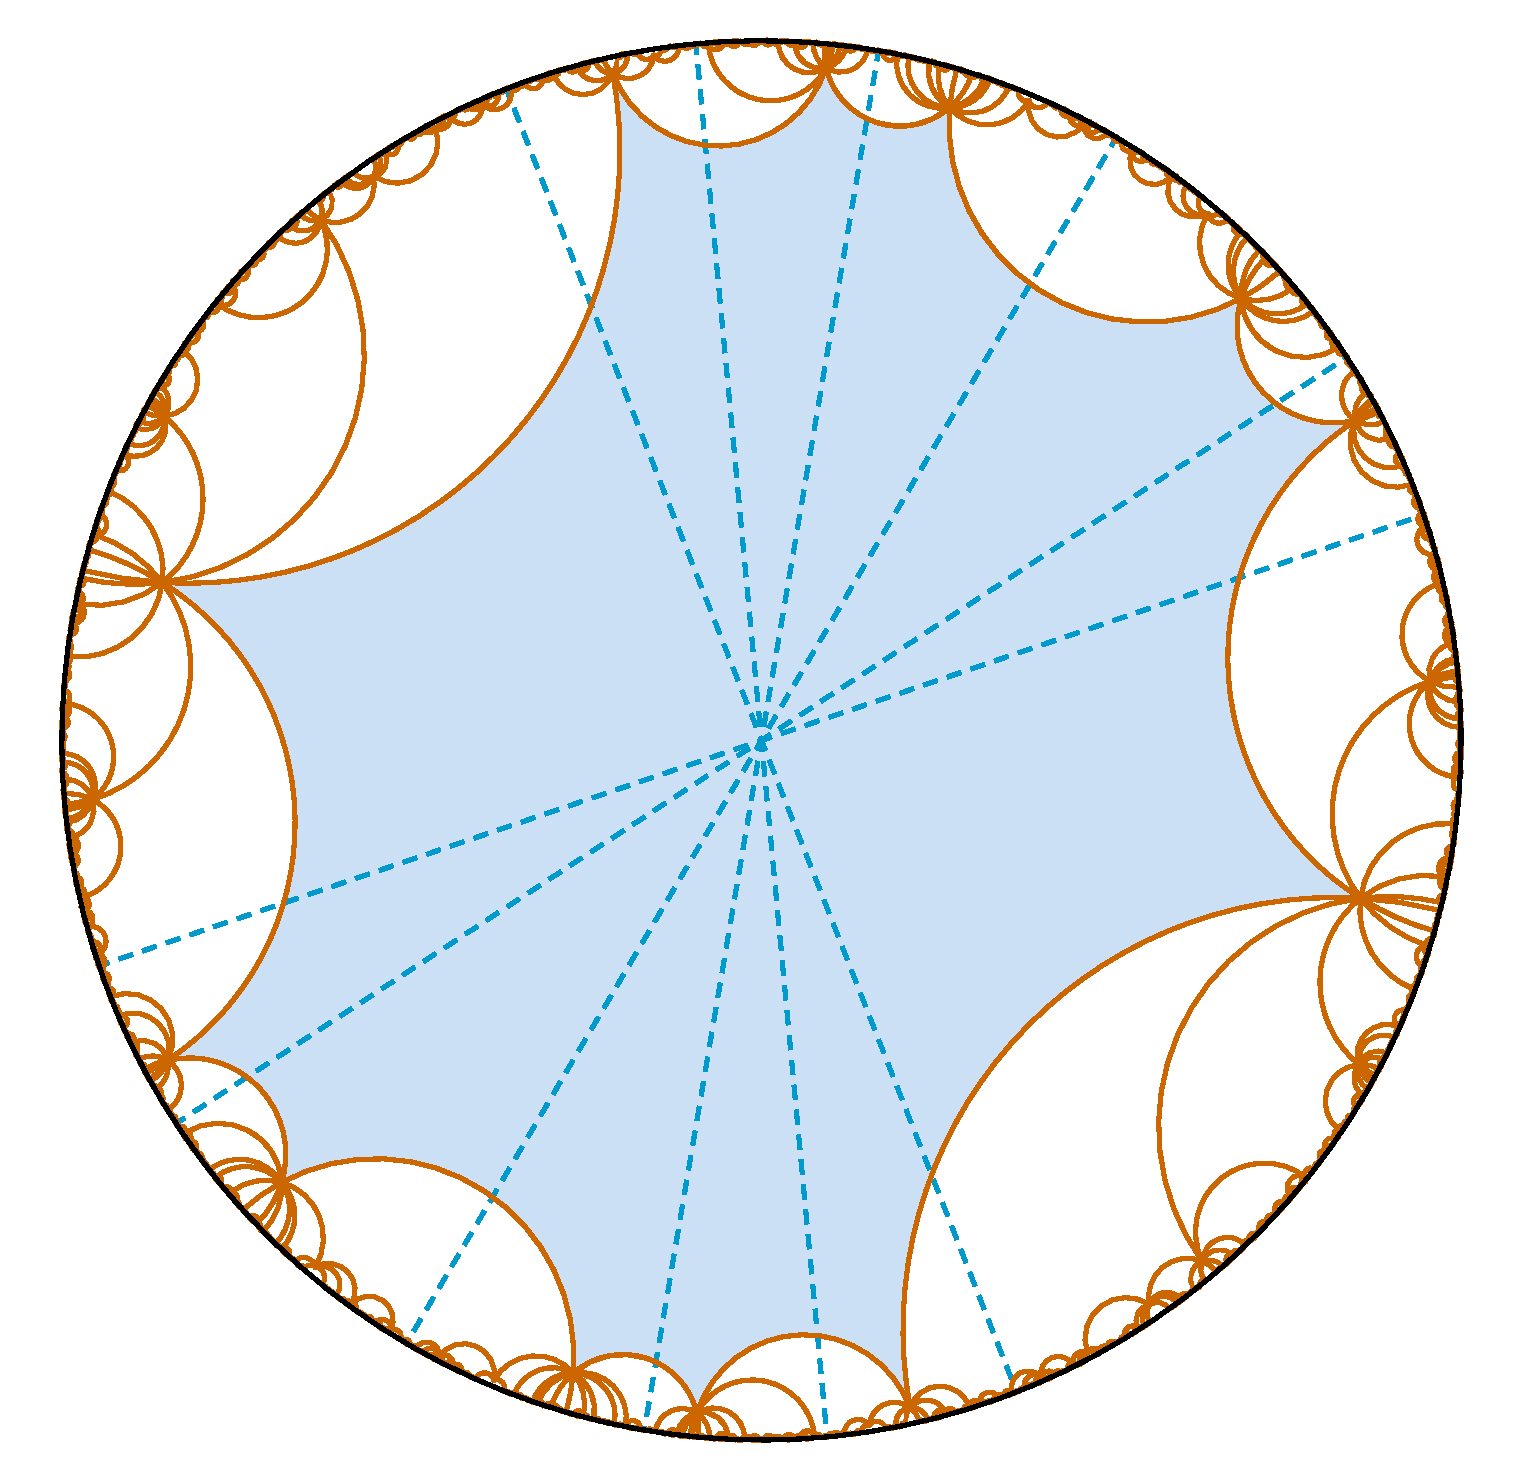
\includegraphics[width=0.35\linewidth]{introduction/hyperelliptic_polygon.pdf}
\caption{A hyperelliptic Riemann surface represented as quotient of the hyperbolic plane, here pictured as the Poincar{\'e} disk model, and a group of hyperbolic motions. The surface is the equivalence class of points with respect to a uniformization group of hyperbolic motions. A fundamental domain (blue area) can be chosen such that the axes of the motions (dashed blue lines) intersect in a common point. This particular representation is calculated from a discrete hyperelliptic curve, i.e. a doubly covered Riemann sphere branched at $2g + 2$ points, see Section~\ref{sec:branched_coverings}.}
\label{fig:intro_hyperelliptic_surface}
\end{figure}

The work is divided into three parts. Part~\ref{part:uniformization} covers discrete uniformization of Riemann surfaces via conformal equivalence of triangle meshes. We build onto the variational principles established in \cite{Bobenko2010} and present a wealth of constructions and examples. Taken from smooth differential geometry and translated to the discrete setting we observe properties known from classic theorems. This culminates in a new conjecture about hyperelliptic Riemann surfaces. A Riemann surface is hyperelliptic if and only if the axes of the uniformization group elements meet in a common point for a suitable representation of the group, see Figure~\ref{fig:intro_hyperelliptic_surface}.

In Part~\ref{part:applications} we present three applications of discrete conformal mapping in the context of architectural geometry. In Chapter~\ref{chp:periodic_conformal_maps} we calculate regular patterns on architectural facade geometries with a period. In Chapter~\ref{chp:quasiisothermic} we exploit the fact that isothermic surfaces possess a unique conformal curvature line parametrization to create meshes with planar quadrilaterals and touching incircles. This problem is formulated as a boundary value problem. Starting from there we conjecture the existence of a discrete ellipsoid. In Chapter~\ref{chp:gridshells} we use discrete conformal maps as initialization for discrete Tschebyshev meshes, i.e., meshes with equal edges length. By doing so we control the curvature and intersection angles of parameter curves in the resulting gridshell construction.

The third part of this work introduces the reader to the software framework build for calculation with discrete surfaces and in particular with discrete conformal mappings, see Chapter~\ref{chp:conformallab} {\sc ConformalLab}, and discrete surface optimization, Chapter~\ref{chp:varylab} {\sc VaryLab}. The author has implemented the software packages {\sc HalfEdge} and {\sc HalfEdgeTools}, see Chapter~\ref{chp:halfedge}, designed as a general tool for the calculation with discrete surfaces. Together with the user interface library {\sc JRWorkspace}, Chapter~\ref{chp:jrworkspace}, it constitutes a flexible framework for the creation of research applications in the context of discrete differential geometry. 

The digital data accompanying this work includes most of the examples presented in Part~\ref{part:uniformization} and the main files for the architectural applications. Additionally we give the current state of the source code of the programming framework presented in Part~\ref{part:implementation}. Its organization is presented in the Appendix.

\subfilebibliography
\end{document}

%%% Local Variables:
%%% TeX-master: "Thesis.tex"
%%% End: